\chapter{Simulation Validations}\label{chapter4}
\subsubsection{Simulation Setup}
To verify the estimation performance of the two proposed flux estimators, the `\texttt{Three-phase PMSM Traction Drive}' example for the 35kW IPMSM provided by MATLAB/Simulink (R2023b), which utilizes the FEM-parameterized PMSM library, was used. Figure \ref{Fig:4.1} shows the overall simulation environment of the PMSM, where the controller was modified for the flux linkage estimator and the FCS-MPC current controller. The simulation specifications and flux linkage maps are listed in Table \ref{Tab4.1} and shown in Fig.\ref{Fig:4.2}. 
To implement FCS-MPC-based current control, \begin{figure}[h]
    \centering
    \includegraphics[scale=0.53]{chapters/Fig4.1.pdf}
    \caption{MATLAB/Simulink simulation environment for IPMSM control}
    \label{Fig:4.1}
\end{figure}a numerical reference generator presented in \cite{c1_2} was used to convert the torque command into current references. Additionally, the sampling time for the sensors was set to 20 kHz, and the sampling time for the flux linkage estimator and FCS-MPC switching calculation was set to 40 kHz. The period for the torque generator was set to 1 kHz. These control periods were determined using the \texttt{"state flow"} library provided by MATLAB/Simulink. 
\begin{table}[t]
\caption{Specifications of the IPMSM Drive}\label{Tab4.1}
\centering
\begin{tabular}{l r}
\toprule
\hline
\textbf{Parameter} & \textbf{Value}  \\ \midrule
Base speed & 2000 rpm \\
Maximum torque & 180 Nm\\
DC-link voltage ($U_{\text{dc}}$) & 325 V \\
Maximum stator current ($I_{\text{max}}$) & 350 A \\
Rotor Inertia & 0.1234 kg\,m$^2$ \\
Number of pole pairs ($n_p$) & 8\\
Stator winding resistance ($R_s$) & 10.9 m$\Omega$\\
Time sampling ($T_s$) & 25 $\mu$s \\
\hline
\bottomrule
\end{tabular}
\end{table}
\begin{figure}[t]
    \centering
    \begin{subfigure}[c]{0.47\textwidth}
        \centering
        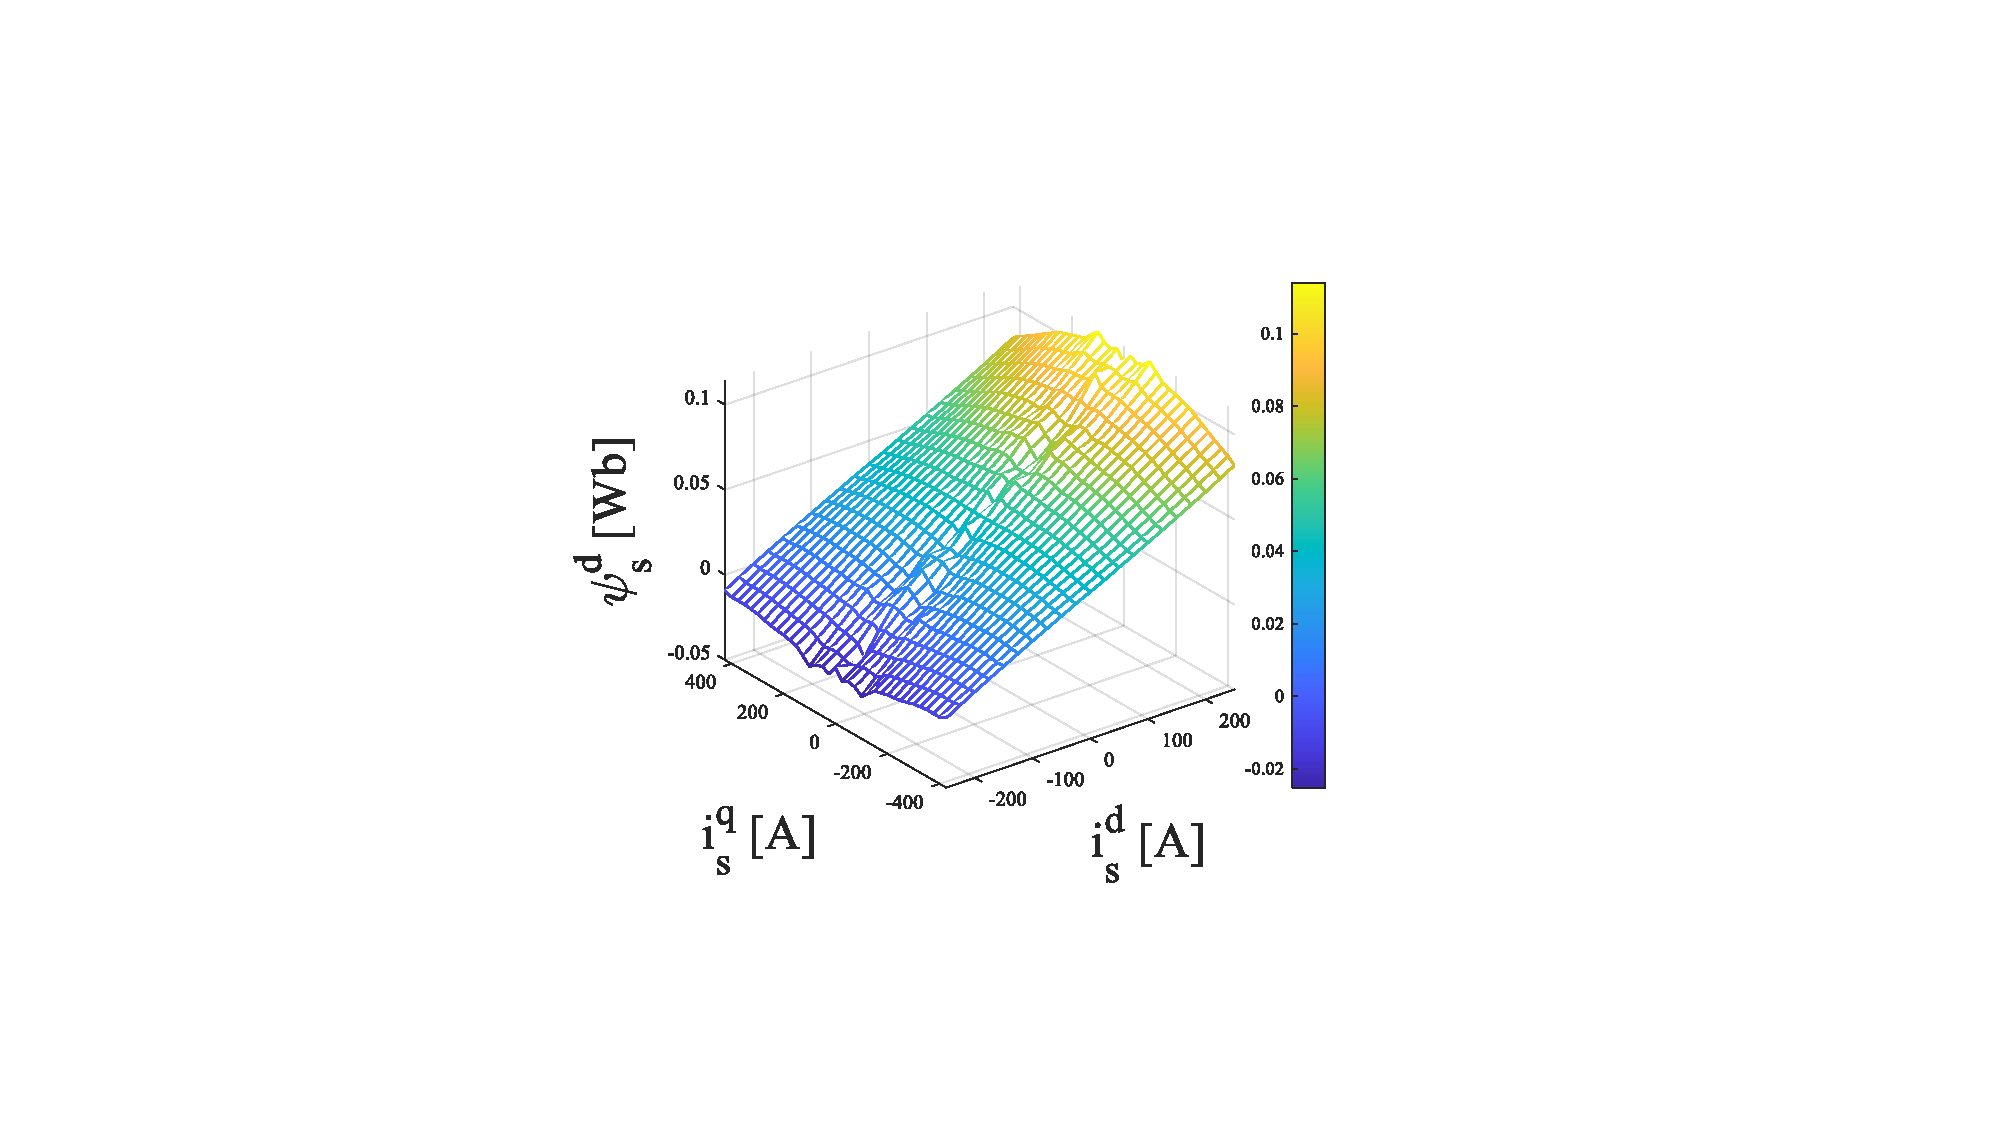
\includegraphics[scale=0.5]{chapters/Fig4.2a.pdf}
        \caption{}
        \label{Fig:4.2a}
    \end{subfigure}
    \hfill
    \begin{subfigure}[c]{0.47\textwidth}
        \centering
        \includegraphics[scale=0.5]{chapters/Fig4.2b.pdf}
        \caption{}
        \label{Fig:4.2b}
    \end{subfigure}
    \caption{Nonlinear flux linkage maps of the IPMSM (a) $d$-axis and (b) $q$-axis.}
    \label{Fig:4.2}
\end{figure}

To determine the gain matrices ${{\boldsymbol{F}({\omega}_{r})}}$ of all state observers (DOB-FLE, ESO-FLE, and IE-PU-FLE) used for simulation verification, a robust pole assignment method \cite{c3.2_3} was utilized to place the system poles at the desired (stable) eigenvalues. This can be easily achieved by using the MATLAB command \texttt{"place"} to calculate the gain matrix ${{\boldsymbol{F}({\omega}_{r})}}$. Additionally, the feedback gain matrix ${{\boldsymbol{F}({\omega}_{r})}}$ was designed so that the bandwidth of the stable eigenvalues of the matrix ${{\boldsymbol{A}}({\omega}_{r})} - {{\boldsymbol{F}({\omega}_{r})}} {{\boldsymbol{C}}}$ is approximately 100 Hz (628 rad/s) at a constant mechanical speed of 500 RPM for all flux linkage estimators. This bandwidth was chosen to be about twice the settling time (50 Hz) of the torque reference command, considering the estimation performance.

\section{Validation of the Proposed ESO-FLE}
The simulation scenarios for verifying the estimation performance of the proposed ESO-FLE are as follows: (i) The estimation performance was verified using nominal inductance ($\mathbf{L}^{dq}_{s,0}$), with the mechanical speed varying from 200 RPM to 1300 RPM and the torque changing from -180 Nm to 180 Nm (In Fig. \ref{Fig:4.3}). (ii) The transient estimation performance was examined using the guessed nominal inductance ($\hat{\mathbf{L}}^{dq}_{s,0}:=0.5\mathbf{L}^{dq}_{s,0}$), with a fixed speed of 500 RPM \begin{table}[h]
\caption{Observer parameters for ESO-FLE}\label{Tab4.2}
\centering
\begin{tabular}{l c}
\hline
\textbf{Parameter} & \textbf{Value}  \\ \midrule
Feedback gain matrix & $\mathbf{F}(419\frac{\text{rad}}{\text{s}})=\begin{bmatrix}
    0.0782 & -0.6481\\
    0.6565 & 0.0919\\
    -0.4008 & -0.7540\\
    0.7599 & -0.3822\\
    -1.4033 & -162.11\\
    166.06 & 1.2415
\end{bmatrix}$\\
\\
Nominal inductance & $\mathbf{L}^{dq}_{s,0}=\begin{bmatrix}
    0.25 & 0\\
    0 & 0.28
\end{bmatrix}$mH\\
\\
\textit{Guessed} nominal inductance & $\hat{\mathbf{L}} ^{dq}_{s,0}= 0.5\times\begin{bmatrix}
    0.25 & 0\\
    0 & 0.28
\end{bmatrix}$mH\\
\\
\hline
\end{tabular}
\end{table}and the torque increasing from 0 to 180 Nm (In Fig. \ref{Fig:4.9}). In all scenarios, a gain matrix selected for a constant mechanical speed of 500 RPM was used for the estimation. The observer parameters used to verify the estimation performance of the proposed ESO-FLE are listed in Tab. \ref{Tab4.2} 

Figure \ref{Fig:4.3} shows the flux linkage estimates, their estimation errors \(\boldsymbol{e}_s := \boldsymbol{\psi}^{dq}_s - \hat{\boldsymbol{\psi}}^{dq}_s\), and the operating conditions of the proposed ESO-FLE. At $t = 0.05$ seconds, when the electrical torque starts increasing to 180 Nm, a large spike-like estimation error occurred in the flux estimates during the transient state (during $t=0.05$ s and $t=0.07$ s). This is because the observer gain matrix \(\mathbf{F}(\omega_r)\) was designed for a constant speed of 500 rpm rather than varying with the mechanical speed, making the observer gain sensitive in the low-speed region and affecting the estimation performance. However, above 200 RPM, the flux linkage estimates closely tracked their true values under dynamic operating conditions across a wide range of torque (-180 Nm to 180 Nm) and speed (200 RPM to 1300 RPM). Thus, the simulation results in Fig. \ref{Fig:4.3} demonstrated that the proposed ESO-FLE shows good estimation performance in both transient and steady states over a wide operating range using nominal inductance, thereby validating its effectiveness.

Figure \ref{Fig:4.9a} shows the transient estimation performance results at a constant speed of 500 RPM using the guessed nominal inductance, and Figure \ref{Fig:4.9b} shows the estimation error norm $||\mathbf{e}_s||$, which quantitatively represents the estimation performance. Here, because the finite control set MPC method directly determines the $d$-axis and $q$-axis voltage inputs for the $d$-axis and $q$-axis current references, respectively, it seems that the flux estimates include significant switching ripples in their estimation error norms. \begin{figure}[!h]
    \centering
    \includegraphics[scale=2.1]{chapters/Fig4.3.pdf}
    \caption{Flux linkage estimates of the proposed ESO-FLE}
    \label{Fig:4.3}
\end{figure} \begin{figure}[h!]
    \centering
    \begin{subfigure}[c]{1.0\columnwidth}
        \centering
        \includegraphics[scale=0.48]{chapters/Fig4.9a.pdf}
        \caption{}
        \label{Fig:4.9a}
    \end{subfigure}
    \vfill
    \begin{subfigure}[c]{1.0\columnwidth}
        \centering
        \includegraphics[scale=0.48]{chapters/Fig4.9b.pdf}
        \caption{}
        \label{Fig:4.9b}
    \end{subfigure}
    \caption{Transient estimation performance of the proposed ESO-FLE (a) Flux linkage estimates (b) The corresponding estimation error norm $||\mathbf{e}_s||$.}
    \label{Fig:4.9}
\end{figure}However, as shown in the simulation results of Fig. \ref{Fig:4.9a} and Fig. \ref{Fig:4.9b}, the improved transient estimation performance despite parameter inaccuracies indicates that assuming nonlinear flux linkage $\Delta\mathbf{\psi}^{dq}_s$ as ramp disturbance signals with a constant slope is reasonable.

\section{Validation of the Proposed IE-PU-FLE}
Likewise, the ESO-FLE, the simulation scenarios for verifying the estimation performance of the proposed IE-PU-FLE are as follows: (i) The estimation performance was verified using $q$-axis nominal inductance ($L^q_{s,0}$) under two conditions with a constant mechanical speed of 500 RPM while the torque increased from 0 to 180 Nm, and with the mechanical speed varying from 200 RPM to 1800 RPM while the torque changed from -180 Nm to 180 Nm (In Figs. \ref{Fig:4.4}, \ref{Fig:4.5} and \ref{Fig:4.6}). (ii) The transient estimation performance was examined by updating the inaccurate initial nominal inductance ($\hat L^q_{s,0}:=2L^{q}_{s,0}$) to the actual inductance while the mechanical speed increased from 200 RPM to 1200 RPM and the torque frequently changed from -180 Nm to 180 Nm (In Figs. \ref{Fig:4.7} and \ref{Fig:4.8}). In all scenarios, a gain matrix selected for a constant mechanical speed of 500 RPM was used for IE-PU-FLE. The observer parameters used to verify the estimation performance of the proposed ESO-FLE are listed in Table \ref{Tab4.3}.

\begin{table}[h]
\caption{Observer parameters for IE-PU-FLE}\label{Tab4.3}
\centering
\begin{tabular}{l c}
\hline
\textbf{Parameter} & \textbf{Value}  \\ \midrule
Feedback gain matrix & $\mathbf{F}(419\frac{\text{rad}}{\text{s}})=\begin{bmatrix}
    1271.25 & 564.01\\
    -545.63 & 1271.10\\
    0.012 & -977.27\\
    964.47 & 8.82
\end{bmatrix}$\\
\\
Nominal inductance & $L^{q}_{s,0}=0.28$mH\\
\\
\textit{Guessed} nominal inductance & $\hat{L} ^{q}_{s,0}= 2\times0.28$mH
\\
\\
Forgetting factor & $\beta = 600$
\\
\\
\hline
\end{tabular}
\end{table}
\newpage
\begin{figure}[h]
    \centering
    \begin{subfigure}[b]{0.80\textwidth}
        \centering
        \includegraphics[scale=0.57]{chapters/Fig4.4a.pdf}
        \caption{}
        \label{Fig:4.4a}
    \end{subfigure}
    \vfill
    \begin{subfigure}[b]{0.80\textwidth}
        \centering
        \includegraphics[scale=0.57]{chapters/Fig4.4b.pdf}
        \caption{}
        \label{Fig:4.4b}
    \end{subfigure}
    \caption{Stator flux linkage estimates (a) in the $(\alpha,\beta)$-reference frame and (b) in the $(d,q)$-reference frame without using the integration error estimator.}
    \label{Fig:4.4}
\end{figure}

Figures \ref{Fig:4.4} and \ref{Fig:4.5} show the estimation results without and with the integration error estimator, respectively. Figure \ref{Fig:4.4a} demonstrates that the flux estimates had offsets $\mathbf{O}^{\alpha\beta}_s$ in the ($\alpha$,$\beta$)-reference frame due to inaccurate integration because the integration error was not estimated and compensated. \begin{figure}[H]
    \centering
    \begin{subfigure}[b]{0.80\textwidth}
        \centering
        \includegraphics[scale=0.55]{chapters/Fig4.5a.pdf}
        \caption{}
        \label{Fig:4.5a}
    \end{subfigure}
    \vfill
    \begin{subfigure}[b]{0.80\textwidth}
        \centering
        \includegraphics[scale=0.55]{chapters/Fig4.5b.pdf}
        \caption{}
        \label{Fig:4.5b}
    \end{subfigure}
        \vfill
    \begin{subfigure}[b]{0.80\textwidth}
        \centering
        \includegraphics[scale=0.55]{chapters/Fig4.5c.pdf}
        \caption{}
        \label{Fig:4.5c}
    \end{subfigure}
    \caption{Stator flux linkage estimates (a) in the $(\alpha,\beta)$-reference frame and (b) in the $(d,q)$-reference frame using the integration error estimator. (c) The corresponding integration estimates}
    \label{Fig:4.5}
\end{figure}Figure \ref{Fig:4.4b} shows that these offsets in the ($\alpha$,$\beta$)-reference frame were transformed into oscillating components in the rotating ($d$,$q$)-reference frame, which deteriorated the estimation performance. In contrast, Figure \ref{Fig:4.5a} shows that using the integration error estimator, the integration error was compensated, allowing the estimates in the ($\alpha$,$\beta$)-reference frame to accurately track the true values. Consequently, as shown in Fig. \ref{Fig:4.5b}, the estimates in the ($d$,$q$)-reference frame also accurately tracked the true values. This accurate estimation was possible because the integration error was estimated online and compensated in the integration result, as shown in Fig. \ref{Fig:4.5c}.

Figure \ref{Fig:4.6} shows the flux linkage estimates and integration error estimates ($\hat{\boldsymbol{\psi}}^{dq}_s$ and $\hat{\mathbf{O}}^{\alpha\beta}_s$) under different operating conditions for the proposed IE-PU-FLE. At $t=0.05$ seconds, when the mechanical speed was 200 RPM and the torque increased from 0 to 180 Nm, there was an overshoot in the flux estimates due to the observer gain matrix being designed for a fixed speed of 500 RPM, causing estimation errors. However, excluding the low-speed region (after t = 0.07), even under varying torque conditions, the proposed IE-PU-FLE accurately estimated and compensated for the integration error with the fixed observer gain, demonstrating excellent estimation performance in both transient and steady states. Therefore, it is demonstrated that the proposed IE-PU-FLE significantly improves the transient and steady-state performance with the nominal inductance parameter over a wide range of speeds.

\begin{figure}[H]
    \centering
    \includegraphics[scale=0.50]{chapters/Fig4.6.pdf}
    \caption{Stator flux linkage and integration error estimates in the ($d$,$q$)-reference frame}
    \label{Fig:4.6}
\end{figure}
\newpage
\begin{figure}[H]
    \centering
    \includegraphics[scale=0.65]{chapters/Fig4.7.pdf}
    \caption{Proposed stator flux linkage estimator based on the integration error estimator}
    \label{Fig:4.7}
\end{figure}

Figure \ref{Fig:4.7} shows the flux estimates ($\hat{\boldsymbol{\psi}}^{dq}_s$) and $q$-axis inductance estimates ($\hat{L}^{q}_s$) for the proposed IE-PU-FLE under different operating conditions when the nominal inductance parameters are inaccurate. Where the mechanical speed increased linearly from 200 RPM to 1200 RPM, the initial $q$-axis inductance was twice the actual value from $t=0$ to $t=0.02$. However, from $t=0.02$, as the torque (current) decreased to -180 Nm, the inductance estimate became closer to the actual value, thereby reducing the estimation error of the flux estimate in transient state. Additionally, when the torque changed periodically, the $q$-axis inductance was updated online, improving transient estimation performance. Therefore, the proposed IE-PU-FLE method, based on an adaptive observer, was verified through extensive simulation scenarios to be robust against parameter variations by updating the observer's $q$-axis inductance to the actual value online across a wide range of operating conditions, thereby enhancing both transient and steady-state estimation performance.

\section{Performance Comparison between DOB-FLE and the Proposed Estimators}

To compare the flux estimation performance of the proposed ESO-FLE and IE-PU-FLE with the existing DOB-FLE, the gain matrix ${{\boldsymbol{F}({\omega}_{r})}}$ was designed to have a bandwidth of approximately 100 Hz for the observer feedback matrix ${{\boldsymbol{A}}({\omega}_{r})} - {{\boldsymbol{F}({\omega}_{r})}} {{\boldsymbol{C}}}$ at a constant mechanical speed of 500 RPM. In this setup, the nominal inductance parameters of the observers were inaccurately set to half of the actual values for each case to compare the transient estimation performance.

Figure \ref{Fig:4.8} shows the stator flux linkage estimates and estimation error norms of IE-PU-FLE, ESO-FLE, and DOB-FLE in the ($d$,$q$)-reference frame, as well as the $q$-axis inductance estimate of IE-PU-FLE, as the torque changes from  -180 Nm to 180 Nm and mechanical speed varies from 200 RPM to 1000 RPM. 

The estimates of DOB-FLE did not exhibit estimation errors in steady state, but in transient state (especially under low-speed conditions between 0.05 seconds and 0.07 seconds), flux estimation errors occurred and did not converge to the true values. Because DOB-FLE assumes the nonlinear flux $\Delta\boldsymbol{\psi}^{dq}_s$ as step signals, it can only satisfy estimation performance in steady state. However, in the transient state, it fails to account for additional disturbances caused by parameter inaccuracies, resulting in significant estimation errors in the flux estimates. \begin{figure}[!t]
    \centering
    \includegraphics[scale=0.58]{chapters/Fig4.8.pdf}
    \caption{Estimation performance comparison of the proposed ESO-FLE, IE-PU-FLE, and DOB-FLE. }
    \label{Fig:4.8}
\end{figure} 

By contrast, as seen in Fig.\ref{Fig:4.8}, ESO-FLE demonstrated improved transient performance compared to DOB-FLE. This enhancement is attributed to ESO-FLE's approach of treating the nonlinear flux term $\Delta\boldsymbol{\psi}^{dq}_s$ as time-varying ramp disturbance signals, unlike DOB-FLE, which assumes these disturbances to be constants. It is also evident that only the estimation error of ESO-FLE decreased compared to DOB-FLE during transient states.

Furthermore, IE-PU-FLE demonstrated significant improvements in both transient and steady-state estimation performance by using RLS to update the $q$-axis inductance parameter in real-time and employing an adaptive observer to continuously compensate for parameter errors, thereby improving the estimation performance, even when the initial inductance parameters were inaccurately set. However, as shown in the $q$-axis inductance estimates between $t=0.02$ and $0.05$, if the input signal does not satisfy the PE condition or if the input signals are insufficient (i.e. $d$-$q$ axis currents are small), estimation errors in the inductance estimates may occur.




